%auto-ignore
\documentclass[tikz]{standalone}

\usetikzlibrary{calc}

\begin{document}
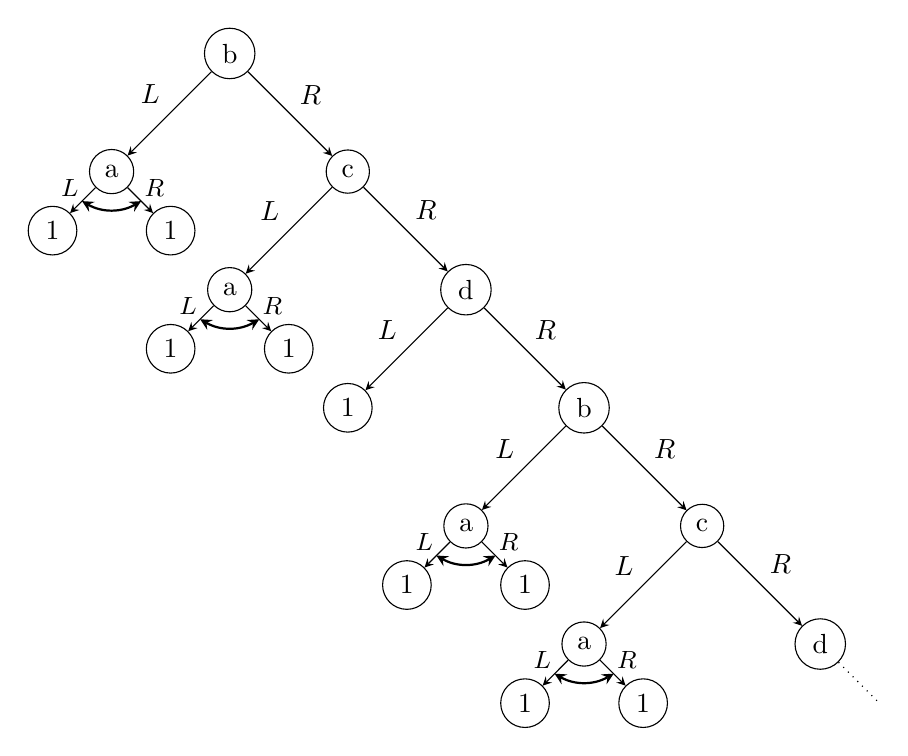
\begin{tikzpicture}[scale=1.5,>=stealth]

\node [circle,draw=black] (n0) at ( 0,  0) {b};
\node [circle,draw=black] (n1) at ( 1, -1) {c};
\node [circle,draw=black] (n2) at ( 2, -2) {d};
\node [circle,draw=black] (n3) at ( 3, -3) {b};
\node [circle,draw=black] (n4) at ( 4, -4) {c};
\node [circle,draw=black] (n5) at ( 5, -5) {d};

\node [circle,draw=black] (m1) at (-1, -1) {a};
\node [circle,draw=black] (m2) at ( 0, -2) {a};
\node [circle,draw=black] (m3) at ( 1, -3) {1};
\node [circle,draw=black] (m4) at ( 2, -4) {a};
\node [circle,draw=black] (m5) at ( 3, -5) {a};


\node [circle,draw=black] (m11) at (-1-0.5, -1-0.5) {1};
\node [circle,draw=black] (m12) at (-1+0.5, -1-0.5) {1};
\draw [<->,thick] ($(m1)!0.5!(m11)$) to [bend right] ($(m1)!0.5!(m12)$);
\draw [->] (m1) to node [above left=-0.2em] {\small$L$} (m11);
\draw [->] (m1) to node [above right=-0.2em] {\small$R$} (m12);

\node [circle,draw=black] (m21) at ($(m2)+(-0.5,-0.5)$) {1};
\node [circle,draw=black] (m22) at ($(m2)+( 0.5,-0.5)$) {1};
\draw [<->,thick] ($(m2)!0.5!(m21)$) to [bend right] ($(m2)!0.5!(m22)$);
\draw [->] (m2) to node [above left=-0.2em] {\small$L$} (m21);
\draw [->] (m2) to node [above right=-0.2em] {\small$R$} (m22);


\node [circle,draw=black] (m41) at ($(m4)+(-0.5,-0.5)$) {1};
\node [circle,draw=black] (m42) at ($(m4)+( 0.5,-0.5)$) {1};
\draw [<->,thick] ($(m4)!0.5!(m41)$) to [bend right] ($(m4)!0.5!(m42)$);
\draw [->] (m4) to node [above left=-0.2em] {\small$L$} (m41);
\draw [->] (m4) to node [above right=-0.2em] {\small$R$} (m42);

\node [circle,draw=black] (m51) at ($(m5)+(-0.5,-0.5)$) {1};
\node [circle,draw=black] (m52) at ($(m5)+( 0.5,-0.5)$) {1};
\draw [<->,thick] ($(m5)!0.5!(m51)$) to [bend right] ($(m5)!0.5!(m52)$);
\draw [->] (m5) to node [above left=-0.2em] {\small$L$} (m51);
\draw [->] (m5) to node [above right=-0.2em] {\small$R$} (m52);

\draw [dotted] (n5) to ($(n5)+(0.5,-0.5)$);

\path[->]
	(n0) edge node [above right] {$R$} (n1)
	edge node [above left] {$L$} (m1)
	(n1) edge node [above right] {$R$} (n2)
	edge node [above left] {$L$} (m2)
	(n2) edge node [above right] {$R$} (n3)
	edge node [above left] {$L$} (m3)
	(n3) edge node [above right] {$R$} (n4)
	edge node [above left] {$L$} (m4)
	(n4) edge node [above right] {$R$} (n5)
	edge node [above left] {$L$} (m5)
;

\end{tikzpicture}
\end{document}